\documentclass{article}
\usepackage[utf8]{inputenc}
\usepackage{titling}
\usepackage{graphicx}
\usepackage[colorlinks=true,linkcolor=blue, urlcolor = blue]{hyperref}
\usepackage[spanish]{babel}
\DeclareUnicodeCharacter{301}{~}
\usepackage{url}


\title{BIG DATA, BUSINESS INTELLIGENCE Y ANÁLISIS DE DATOS}
\author{Cristina Díaz García}
\date{October 2018}

\renewcommand\maketitlehooka{\null\mbox{}\vfill}
\renewcommand\maketitlehookd{\vfill\null}


\begin{document}

\addcontentsline{toc}{section}{Índice general}

\begin{titlingpage}
\maketitle
\end{titlingpage}

\newpage

\tableofcontents

\newpage

\section{Introduction}
La tecnología no para de avanzar a un ritmo vertiginoso: tenemos mucha información, queremos almacenarla y sacar provecho de ella. Es por ello que en las próximas páginas definiremos conceptos como minería de datos, business intelligence, análisis de sentimientos, big data, análisis de datos y su visualización y cuadro de mando integral, cuya relevancia es cada vez mayor.

\section{Descripción de los conceptos}
Empezaremos describiendo de manera muy simple todos los conceptos, poniendo ejemplos para verlo más fácilmente y relacionándolos con lo visto en clase. Nuestro ejemplo va a ser una papelería de una gran superficie.

El big data es la base sobre la que se sustenta una parte importante de la tecnología de hoy en día: es un conjunto inmenso de datos, tanto que su almacenamiento y su manipulación se hacen costosas, ya sea respecto a los recursos hardwares como a las técnicas tradicionalmente usadas. En nuestro ejemplo, el big data serían todas las compras hechas por todos los clientes.

El business intelligence, en castellano inteligencia de negocio, es la forma de referirse a usar los datos que ese negocio tiene para tomar decisiones más conscientes. En nuestro ejemplo, estas decisiones podrían ser cambiar la localización de ciertos productos, crear nuevos o abrir otra sucursal en otra ciudad. 

El análisis de datos es una de las formas de manipulación de la información, con el que, valga la redundancia, se analizan los datos: se observan, se eliminan datos erróneos o inútiles y se resalta la útil para poder sacar conclusiones. A este análisis le sigue una visualización de datos, es decir, interpretar esos datos, contrastarlos y compararlos para que las conclusiones que se saquen sean las más fieles a la realidad posibles. 

También es común realizar lo que se llama análisis de sentimientos, que consiste en extraer información de redes sociales, foros, webs, comentarios...para así lo que la persona que haya publicado esa información piensa. En nuestro ejemplo, esto sería analizar por los comentarios que los usuarios dejan en nuestra web, en Twitter o en cualquier red social en la que tengamos una cuentra creada, para ver si el nuevo producto está gustando o si nuestra marca obtiene buenas críticas por los influencers. 

Otra de las formas de manipulación de la infomación es la minería de datos. Esto es la extracción de la información y de patrones en ella, es decir, ver a rasgos generales qué información tenemos y cómo organizarla, cómo agruparla para que después podamos extraer fácilmente conclusiones para tomar las decisiones que veamos convenientes.  En nuestro ejemplo, la minería de datos sería analizar todas las transacciones, todas las compras que todos los clientes, y descubrir que las mismas personas que compraban libretas tienden a comprar bolígrafos también, o que las que compran cinta adhesiva también compran tijeras.

A gestionar todas estas tácticas de negocio ayuda el cuadro de mando integral, que es un modelo de gestión para establecer unos objetivos relacionados entre sí, medir el progreso de estos con unos indicadores y fijar un plan de acción para cada uno. Lo más importante de este cuadro es crear y comunicar a toda la empresa cuál va a ser la estrategia a seguir.

En la siguiente imagen se muestra este cuadro:

\begin{flushleft}
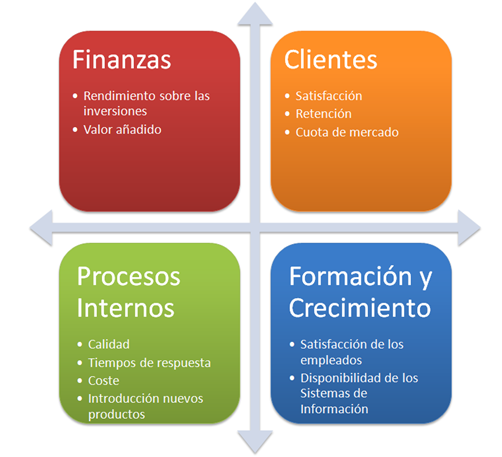
\includegraphics[scale=0.7]{Cuadro-de-Mando-Integral1.png}
\end{flushleft}

\section{Estudio de software para análisis de datos: Tensorflow}
Tensorflow es una biblioteca de código libre desarrollada por Google. Esta librería trabaja sobre C++ o Python, entre otros, siendo este último el más común, y se usa para realizar calculos numéricos, concretamente, cálculos en los que se basan las redes neuronales.

Para usar esta biblioteca necesitaremos Ubuntu 16.04 o posterior, Windows 7 o posterior, macOS Sierra o posterior, aunque entonces no tendríamos Soporte de GPU, o raspbian 9.0 o posterior.

Tendremos que instalar el gestor de paquetes pip, Python y los paquetes de la librería de Tensorflow, y ya se podría empezar a programar en nuestro IDE preferido, haciendo uso de la API que se nos proporciona.




\section{Conclusión personal}
En mi opinión, todas estas estrategias arriba mencionadas son herramientas muy potentes con las que las empresas pueden mejorar su negocio, tanto para su propio beneficio como para beneficio de la personalización de venta de cada cliente y la clientela en general, con su consiguente captación de nuevos clientes y fidelización de los que ya tenían. También es algo que nosotros como clientes tenemos que conocer y tener en cuenta, sabiendo que todo lo que pongamos en Internet , tanto para bueno como para malo, puede ser (y será) analizado.

\begin{thebibliography}{9}
\bibitem{BigData}
Big Data, 
\url{https://www.powerdata.es/big-data}.
\bibitem{BusinessIntelligence}
Business Intelligente, 
\url{https://es.wikipedia.org/wiki/Inteligencia_empresarial}.
\bibitem{DataAnalysis}
Análisis de Datos, 
\url{https://es.wikipedia.org/wiki/An\%C3\%A1lisis_de_datos}.
\bibitem{OpinionMining}
Análisis de Sentimientos, 
\url{https://es.wikipedia.org/wiki/An\%C3\%A1lisis_de_sentimiento}.
\bibitem{OpinionMining2}
Análisis de Sentimientos, 
\url{https://itelligent.es/es/analisis-de-sentimiento/}.
\bibitem{DataMining}
Minería de datos, 
\url{https://es.wikipedia.org/wiki/Miner\%C3\%ADa_de_datos#Ejemplos_de_uso_de_la_miner\%C3\%ADa_de_datos}.
\bibitem{DataMining2}
Minería de datos, 
\url{http://blog.spasolutioncompany.com/otra-rama-de-business-intelligence-la-mineria-de-datos-o-datamining/}.
\bibitem{DataMining3}
Minería de datos, 
\url{https://www.sinnexus.com/business_intelligence/datamining.aspx}.
\bibitem{CuadroMandos}
Cuadro de mandos, 
\url{http://cmigestion.es/cuadro-de-mando-integral/}.
\bibitem{Tensorflow}
Tensorflow, 
\url{https://www.tensorflow.org/?hl=es}.
\end{thebibliography}



\end{document}